%%%%%%%%%%%%%%%%%%%%%%%%%%%%%%%%%%%%%%%%%%%%%%%%%%%%%%%%%%%%%%%%%%%%%%%%%%%%%%%
% bc.tex - Bachelor thesis                                                    %
% Subject: bc_emu - portable video game emulator                              %
% Chapter: Implementace                                                       %
% Author: Ondrej Balaz <ondra@blami.net>                                      %
%%%%%%%%%%%%%%%%%%%%%%%%%%%%%%%%%%%%%%%%%%%%%%%%%%%%%%%%%%%%%%%%%%%%%%%%%%%%%%%

\chapter{Implementace}\label{chap:impl}

Implementace spočívá v převodu navržené architektury do podoby spustitelného
kódu. Způsob jakým jsou jednotlivé části programu implementovány je dán volbou
programovacího jazyka a knihoven popsanou v sekci~\ref{chap:impl_env} této
kapitoly, ale také použitím specifických implementačních technik a konvencí
popsaných v sekci~\ref{chap:impl_techniques}.

Následující sekce kapitoly rámcově rozebírají základní myšlenky použité při
implementaci programového jádra (sekce~\ref{chap:impl_program}), modulu
emulátoru systému NEC PCEngine (sekce~\ref{chap:impl_pce}) a modulů
uživatelských rozhraní libSDL (sekce~\ref{chap:impl_sdl}) a libSDL s podporou
OpenGL (sekce~\ref{chap:impl_sdlgl}).

K podrobnějšímu studiu implementace poslouží zdrojový kód programu, který je
okomentován a psán tak, aby byl co nejvíce čitelný. Tam kde je to vhodné jsou v
kódu (hlavně emulátoru systému NEC PCEngine) uvedeny i části specifikace.
Veškeré komentáře v kódu jsou zpracovatelné systémem Doxygen~\cite{wwwDoxygen}
do přehledné programátorské dokumentace.

Kapitolu uzavírá sekce~\ref{chap:impl_cmake}, která se věnuje použití
sestavovacího systému CMake za účelem konfigurace sestavení a sestavení
programu.

% -----------------------------------------------------------------------------
% Implementacni prostredi
% -----------------------------------------------------------------------------

\section{Implementační prostředí}\label{chap:impl_env}

Implementace emulátoru je nelehký úkol, který vyžaduje, kromě znalosti
architektury emulovaného systému a jeho asembleru, také dobrou znalost
programovacího jazyka, ve kterém bude implementace probíhat. Nejvhodnějšími
kandidáty z kategorie vyšších programovacích jazyků jsou jazyky C a C++, které
disponují datovým typem ukazatel a dovolují přímou práci s pamětí. Zároveň se
jedná o nejrozšířenější jazyky kompilované do nativního kódu cílové platformy.

%
% Programovaci jazyk
%

\subsection{Programovací jazyk}\label{chap:impl_env_lang}

Pro implementaci programu byl z nabízené dvojice programovacích jazyků C a C++
zvolen programovací jazyk C. Toto rozhodnutí je založeno na mých zkušenostech s
touto dvojící programovacích jazyků, ze kterých ovládám více právě programovací
jazyk C.

Ačkoliv je architektura programu navržena částečně objektově, zdaleka nenachází
plné využití možností objektového programování (rozsáhlé abstrakce, složitá
hierarchie tříd vyžadující komplexní využití dědičnosti atd.). Možnosti, které
z tohoto přístupu k programování využívá lze bez větších problémů implementovat
i v jazyce C při dodržení určitých postupů a konvencí, o kterých podrobně
pojednává např.~\cite{Schreiner94}.

Programovací jazyk C má navíc několik vlastností, které ulehčí přenositelnost
výsledného řešení na případné méně standardní platformy. Jedná se o:

\begin{itemize}
\item jazyk C má oproti jazyku C++ méně běhových závislostí, což ho favorizuje
	v případě programování nízkoúrovňových systémů, vestavěných zařízení apod.,
	na která by program mohl být v budoucnu přenášen.

\item jazyk C neprovádí transformaci jmen symbolů, což je velice užitečné při
	např. při lazení a optimalizacích na úrovni assemblerového kódu programu.

\item jazyk C umožňuje, narozdíl od jazyka C++ uložení polí proměnné délky na
	zásobník, kde je alokace velice rychlá. Na některých platformách by toto
	mohlo posloužit k uložení kritických míst emulované paměti.
\end{itemize}

%
% Knihovny a nastroje
%

\subsection{Knihovny a nástroje}\label{chap:impl_env_tools}

K implementaci uživatelského rozhraní je, po vzoru emulátoru Mednafen uvedeného
v rešerši existujících řešení (viz. kapitola~\ref{chap:exist}), použita
knihovna pro tvorbu uživatelských rozhraní libSDL~\cite{wwwlibSDL} a knihovna
pro akcelerovanou grafiku OpenGL~\cite{wwwOpenGL}. Kód používající tyto
knihovny je zapouzdřen do modulu uživatelského rozhraní, nikoliv použit přímo,
a tak může být kdykoliv nahrazen.

Důvodem použití právě těchto knihoven je fakt, že podporují obě, nefunkčními
požadavky, vytyčené platformy (tj. GNU/Linux a Microsoft Windows). Nebude tedy
nutné vytvářet speciální modul uživatelského rozhraní pro každou z těchto
platforem.

Pro konfiguraci sestavení a programu se využívá multiplatformního sestavovacího
nástroje CMake~\cite{wwwCMake}. Více o použití tohoto nástroje je uvedeno v
sekci~\ref{chap:impl_cmake} této kapitoly.

Součástí implementačního prostředí jsou nepochybně i nástroje využité k psaní a
lazení testovacích programů pro procesor HuC6280 - tedy emulátor procesoru 6502
- M6502~\cite{wwwM6502} a assembler pro procesor HuC6280 -
MagicKit~\cite{wwwMagicKit}.

% -----------------------------------------------------------------------------
% Techniky pouzite pri implementaci
% -----------------------------------------------------------------------------

\section{Techniky použité při implementaci}\label{chap:impl_techniques}

Na základě některých nefunkčních požadavků a použití zvolených nástrojů byly
při implementaci použity techniky popsané v následujícím textu.

%
% Objektový přístup a zapouzdření
%

\subsection{Objektový přístup a zapouzdření}\label{chap:impl_techniques_obj}

Objektově orientovaná analýza a návrh software jsou postupy založené na
modelování skutečné reality v programu pomocí tzv. \uv{objektů}. Tyto objekty
jsou zpravidla tvořeny atributy reprezentujícími stav objektu a metodami,
pomocí kterých mohou tento stav ovlivňovat ostatní objekty v modelu. Více o
objektově orientovaném programovacím stylu lze nalézt např v.~\cite{Booch94}.

Analýza a návrh programu byly přirozeně provedeny touto cestou a jednotlivé
jeho části jsou tvořeny objekty, které zapouzdřují činnost těchto částí.

Pro implementaci byl zvolen programovací jazyk C, který, jak už bylo uvedeno,
nemá přímou podporu metodik objektového programování. Nicméně objektově
orientovaná architektura progamu je poměrně jednoduchá a nestaví žádné
závážnější překážky implementaci v tomto jazyce. Pro potřeby implementace
navržené architektury si vystačíme s následujícími technikami:

\begin{description}
\item[třída] - je implementována pomocí datové struktury sdružující všechny
	atributy objektů této třídy a množiny funkcí, které představují
	metody této třídy.

\item[instance] - instance je tvořena ukazatelem na dříve popsanou strukturu
	třídy, které odpovídá. Vytvoření instance proběhne alokací paměti (pomocí
	funkce jazyka C {\em malloc()}) pro tuto strukturu a případně zavoláním
	funkce, která zinicializuje její prvky (konstruktoru). Zrušení instance pak
	proběhne jednoduše uvolněním paměti pro strukturu (pomocí funkce jazyka C
	{\em free()}), případně jemu předcházejícím zavoláním funkce, která provede
	např. uložení dat ze struktury na disk před jejím zánikem (destruktoru).

\item[metoda] - je funkce, jejímž prvním argumentem je vždy ukazatel na konkrétní
	instanci objektu. Tato funkce při svém volání ověří existenci (např. pomocí
	makra jazyka C {\em assert()}) a vykoná činnost.

\item[atribut] - je členská proměnná struktury třídy. Pokud se jedná o ukazatel
	do paměti, měl by destruktor třídy zajistit uvolnění této paměti, pokud je
	to žádoucí.
\end{description}

% TODO priklad kodu tridy? %

Protože návrh programu nepočítá s tím, že by od některé třídy mělo existovat
více instancí, jsou v rámci zdrojového kódu programu instance globální a
nepředávají se metodám. Tento přístup může do budoucna znamenat nepřehlednost
kódu a proto je považován za chybu, která bude odstraněna.

%
% Prenositelnost kodu
%

\subsection{Přenositelnost kódu}

Dalším aspektem úzce spojeným s volbou jazyka C je přenositelnost kódu. Protože
se zdrojový kód programů napsaných v jazyce C překládá přímo do strojového
kódu, není možné přenášet výsledné binární soubory mezi platformami. Místo toho
je nutné pro každou z podporovaných platforem kód přeložit pro ni určeným
překladačem jazyka C.

Kromě toho, že je nutné architektonicky oddělit kód závislý na platformě tak,
jak je to popsáno v kapitole~\ref{chap:anal}, je také nutné vzít v potaz
několik dalších faktorů, které ovlivňují přenositelnost kódu.

% Standardy jazyka C

\subsubsection{Standardy jazyka C}

I přesto, že je množina základních datových typů, knihovních funkcí apod. v
jazyce C předepsaná standardem ANSI C, řada distribucí vývojových nástrojů
jazyka C se liší v jeho výkladu, zavádí jiné pojmenování pro datové typy,
nebo nedefinuje některá makra.

Z toho důvodu existuje soubor {\tt xtypes.h}, kde jsou definovány jednotlivé
datové typy, které by měly být používany v přenositelném kódu. V případě, že
nastane potřeba pro specifický překladač nebo platformu definovat typ jinak,
bude možné to provést podmíněně na jednom místě.

V některých případech navíc není možné, aby překladač odpovídal
standardu\footnote{Např. v případě vývojového prostředí devkitPro pro Nintendo
DS je nutné aby program místo standardní vstupní funkce {\em main()} obsahoval
dvě vstupní funkce z nichž každá je určena pro jeden z dvojice v systému
přítomných procesorů.}. Pro tento případ je i jádro programu rozděleno na dvě
části z nichž jedna implementuje na platformě nezávislý kód a druhá kód na
platformě závislý.

% Endianita

\subsubsection{Endianita}

Endianita (pořadí bajtů) architektury, na které emulátor běží, má v případě
implementace v jazyce C významný dopad na jeho funkčnost. Jak již bylo uvedeno
v kapitole~\ref{chap:anal}, paměť emulovaného systému je reprezentována přímo
pre-alokovanými bloky paměti, uspořádánými dle endianity této architektury.
Emulovaný program ale pracuje s uspořádáním paměti daným endianitou emulovaného
procesoru. V případě že se tyto endianity liší, je nutné na kritických místech
pořadí bajtů obrátit.

Aby těchto míst v kódu programu vznikalo co nejméně, je v souboru {\tt
xtypes.h} zaveden speciální union {\em pair} představující dvojici slov,
jehož definice je následující:

\begin{verbatim}
typedef union {
#ifdef LSB
    struct { uint8 l,h,h2,h3; } b;
    struct { uint16 l,h; } w;
#else
    struct { uint8 h3,h2,h,l; } b;
    struct { uint16 h,l; } w;
#endif
    uint32 d;
} pair;
\end{verbatim}

Pro přístup k celé dvojici slov reprezentované tímto unionem lze použít jeho
prvek {\em d}, pro přístup k hornímu slovu pak prvek {\em w.h} atd. Interní
struktura tohoto unionu je stanovena v okamžiku sestavování programu nastavením
makra {\em LSB}, resp. {\em MSB}, tak aby bylo v kódu přistupováno k žádanému
slovu nebo bajtu.

Jedno z dvojice maker {\em LSB}, {\em MSB}, je vždy nastaveno sestavovacím
systémem CMake na základě informace o endianitě architektury, pro kterou
probíhá sestavení. Podobně jako je použito v případě unionu {\em pair} ho lze
použít na libovolném místě v kódu, kde je nutné zařídit aby data byla správně
reprezentována emulovanému programu a nelze tam union {\em pair} použít (např.
kód VDC nebo PSG).

%
% Konvence dodrzovane v kodu
%

\subsection{Konvence dodržované v kódu}

V kódu jsou pro lepší přehlednost a srozumitelnost dodržovány následující
konvence:

\begin{itemize}
\item názvy identifikátorů jsou tvořeny malými písmeny a podtržítky
\item konstruktory tříd jsou nazvány {\em init}
\item destruktory tříd jsou nazvány {\em shutdown}
\item názvy metod jsou prefixovány názvem příslušné třídy
\item identifikátory v rámci modulu jsou prefixovány názvem modulu
\end{itemize}

% -----------------------------------------------------------------------------
% Program
% -----------------------------------------------------------------------------

\section{Program}\label{chap:impl_program}

Celý program je příznačně nazván {\em bc\_emu}. Skládá se z programového jádra,
platformně závislého kódu pro spuštění z příkazové řádky operačního systému
osobního počítače a následující trojice modulů:

\begin{itemize}
\item emulátoru systému NEC PCEngine ({\em pce})
\item uživatelského rozhraní libSDL ({\em sdl})
\item uživatelského rozhraní libSDL s podporou OpenGL ({\em sdlgl})
\end{itemize}

\subsection{Podpora modulů}

Podpora modulů v programu je implementována pomocí ukazatelů na
funkce~\cite{wwwCFuncPointer}. Při konfiguraci sestavení je systémem CMake
vygenerován soubor {\tt bc\_emu\_modules.c}, který obsahuje dvojici polí
struktur modulů (emulátorů a uživatelských rozhraní) obsahujících ukazatele na
funkce, které tvoří veřejné rozhraní jednotlivých modulů.

Po sestavení má program tyto dvě pole k dispozici a při spuštění jen provede
nastavení globálních ukazatelů podle aktuálně zvolené dvojice modulů. Obecné
rozhraní je dotvořeno trojicí globálních společných datových struktur pro
výměnu dat mezi moduly, definovaných v souboru {\tt interface.h}.

Tento způsob je plně vyhovující pokud budeme předpokládat
statické\footnote{Knihovny jednotlivých modulů jsou přímo připojeny do
binárního souboru programu.} sestavování výsledného programu a fakt, že nikdy
nebude zapotřebí více instancí jednoho typu modulu. Při běžném používaní
programu zamýšleným způsobem budou tyto předpoklady vždy splněny. Pokud by
nastal důvod sestavit program dynamicky\footnote{Knihovny jednotlivých modulů
jsou načítány službou operačního systému při každém spuštění programu.}, bylo by
nutné vhodně rozšířit funkce pro hledání jednotlivých typů modulů v souboru
{\tt module.c}. Podpora více instancí modulu bude vyřešena opravením chyby s
předáváním ukazatele na instanci popsané v
podsekci~\ref{chap:impl_techniques_obj}.

% -----------------------------------------------------------------------------
% Modul emulatoru NEC PCEngine
% -----------------------------------------------------------------------------

\section{Modul emulátoru NEC PCEngine}\label{chap:impl_pce}

Modul emulátoru systému NEC PCEngine je nejvýznamnější částí programu. Obsahuje
veškerý kód zajišťující emulaci jednotlivých částí tohoto systému. Soubory se
zdrojovými kódy modulu jsou umístěny v adresáři {\tt /emu/pce/}.

Nejpodstatnější funkcí celého modulu je bezpochyby funkce {\it pce\_frame()},
která zajišťuje posun o vykreslení jednoho obrazového snímku v emulovaném
programu. Standard NTSC má při kmitočtu 60Hz 59.9 prokládaných snímků tvořených
263-mi řádky.

%
% CPU
%

\subsection{CPU HuC6280}

Veškerá emulace činnosti CPU HuC6280 je zapouzdřena do třídy {\em pce\_cpu}.
Základ této třídy tvoří soubor {\tt cpu\_huc6280.c}, který obsahuje řadu metod
pro samotnou práci s procesorem a soubory instrukční sady: {\tt
cpu\_instr.inc}, {\tt cpu\_instr\_util.inc} a {\tt cpu\_op\_tab.inc}.
Implementace částečně vychází z emulátoru procesoru M6502 Juergena
Buchmuellera.

% Casovani

\subsubsection{Časování}\label{chap:impl_pce_cpu_timing}

Emulátor systému NEC PCEngine je naimplementován tak, aby počet procesorových
cyklů prováděných při vykreslení jednoho řádku snímku odpovídal skutečnému
hardware. Tento počet cyklů lze získat následujícím výpočtem:

$$ n_{cykly} = \frac{f_{VDC}}{n_{snimky} * n_{radky}} = 
	\frac{7,16 * 10^6}{59.9 * 263} \approx 455 $$

kde $f_{VDC}$ je taktovací frekvence VDC~\cite{Schleussinger98}, $n_{snimky}$
je počet prokládaných snímků za sekundu dle standardu NTSC a $n_{radky}$ je
počet řádků tvořících jeden proložený snímek (čitatel je počet vykreslených
řádků za sekundu).

Vzhledem k tomu, že dochází k vykonání přesného počtu procesorových cyklů během
vykreslení řádku a tedy i snímku, bude při počtu snímků za sekundu definovaném
standardem NTSC rychlost emulace věrohodná. To je stav, který je z hlediska
modulu emulátoru vyhovující.

Nicméně pokud není v hlavní programové smyčce, ze které vykreslování
jednotlivých snímků probíhá (soubor {\tt bc\_emu.c}), provedeno omezení počtu
vykreslených snímků na přibližně tuto hodnotu, bude rychlost emulace omezená
pouze rychlostí platformy na které emulátor běží, tedy pravděpodobně příliš
vysoká.

Odstranění této chyby, která není v kódu emulátoru a nelze jí řešit bez použití
služeb knihovny nebo rámce uživatelského rozhraní, případně platformy, je
přenecháno dvojici funkcí {\em frame\_begin()} a {\em frame\_end()} modulu
uživatelského rozhraní (viz.~\ref{chap:impl_sdl_timing}).

% Zpracovani instrukci

\subsubsection{Zpracování instrukcí}

Stěžejní částí emulace CPU HuC6280 je zpracování instrukcí, které probíhá v
rámci metody {\it pce\_cpu\_exec()}. Jejím argumentem je počet procesorových
cyklů k dispozici (pro jeden snímek 455) a návratovou hodnotou je buď záporné
číslo vyjadřující počet chybějících cyklů (instrukce se vykonávají atomicky,
takže byly cykly provedeny navíc), nebo kladné číslo vyjadřující počet cyklů,
který přebyl.

Jednotlivé instrukce jsou implementovány jako inline\footnote{Označení pro
funkce, které překladač jazyka C překládá tak, že v místě volání funkce nevloží
do strojového kódu odskok na rutinu představující kód funkce, ale přímo tento
kód} funkce uspořádané do pole, kde indexem je přímo opkód. Definice těchto
funkcí lze nalézt v přehledné tabulce v souboru {\tt cpu\_op\_tab.inc} a mají
typicky tvar:

\begin{verbatim}
OP(016) { int arg1; cycl_n -= 6;    RD_ZPX;         ASL;        WB_EAZ; }
\end{verbatim}

Kromě deklarace proměnných představujících operandy instrukce a dekrementace
počtu zbývajících cyklů procesoru, tvoří tělo každé funkce implementující
instrukci jedno až tři makra.

Makra s dvoupísmenným prefixem (např. {\tt RD\_ZPX} nebo {\tt WB\_EAZ})
zajišťují přístup do paměti s použitím konkrétního adresního módu. Zdrojový kód
těchto maker je umístěn v souboru {\tt cpu\_instr\_util.inc} a jejich úkolem je
spočítat adresu a obsah paměti na této adrese načíst do připravené proměnné
jako operand instrukce, případně obsah této proměnné nebo některého z registrů
na tuto adresu uložit.

Zbývající makro pak zajišťuje samotnou emulaci instrukce. Zdrojový kód
jednotlivých maker instrukcí je umístěn v souboru {\tt cpu\_instr.inc}.

Z předchozího popisu je zřejmé, že při implementaci cyklického zpracování
instrukcí tímto způsobem stačí v interpretační funkci inkrementovat čítač
programu ({\sf PC}) a zavolat funkci z pole s indexem jeho nové hodnoty.

% Zpracovani preruseni

\subsubsection{Zpracování přerušení}

Implementace emulace CPU HuC6280 bere v potaz zpracování přerušení na všech
linkách přerušení. V případě, že během emulace programu nastane přerušení, je
na příslušné lince nastaven mód \uv{aserce}. Po zpracování přerušení je linka
uvedena zpět do módu \uv{volno}. Stav jednotlivých linek přerušení je uchován
pomocí pole {\it irq\_state[]} v rámci struktury třídy {\it pce\_cpu}.

Zpracování přerušení je implementováno pomocí makra {\it CHECK\_IRQ\_LINES},
které kontroluje stav jednotlivých linek a v případě, že je některá z nich
nastavena na stav \uv{aserce}, zavolá další makro {\it DO\_INTERRUPT} s
vektorem příslušného přerušení v argumentu. Zdrojový kód obou maker je
umístěn v souboru {\tt cpu\_instr\_util.inc}.

Kromě běžného ošetření v rámci emulovaného programu (odskok na vektor přerušení
a spuštění ošetřující rutiny) je navíc volána funkce zpětného volání, na níž
byl nastaven ukazatel pomocí funkce {\it pce\_cpu\_set\_irq\_callback()}. Tato
funkce dostává parametrem identifikátor linky, na které došlo k přerušení.
Tento mechanismus je výhodný např. pro lazení.

%
% VDC + VCE
%

\subsection{VDC HuC6270 + VCE HuC6260}

Emulace zobrazovacího subsystému NEC PCEngine je zajištěna třídami {\it
pce\_vdc} a {\it pce\_vce}. Jejich kód nalezneme v souborech {\tt
vdc\_huc6270.c} a {\tt vce\_huc6260.c}. Výstup obrazových dat je proveden
jejich vykreslením do bitové mapy reprezentované strukturou {\it t\_video},
kterou dále zpracovává modul uživatelského rozhraní.

Vzhledem k tomu, že předmětem práce nebylo studium způsobu zobrazování na
televizoru, emulace VDC i VCE postrádá implementaci řady vlastností (barva
překryvu v prostoru nevyužité obrazovky, nastavení šířky bodových pulzů atd.),
které nijak výrazně neovlivňují funkčnost modulu emulátoru a mohou být doplněny
později.

% VDC

\subsubsection{VDC HuC6270}

Třída {\it pce\_vdc} zajišťuje veškeré vykreslovací operace. Vykreslování
výsledného obrazu do bitové mapy je, stejně jako vykreslování na obrazovku
televizoru v případě skutečného hardware, prováděno po jednotlivých řádcích.
Tento přístup zvyšuje přesnost emulace u programů, které využívají k
synchronizaci přerušení vyvolaných před samotnou {\em vertikální synchronizací}
(např. raster compare, nebo kolize sprajtu 0).

Ústřední funkcí třídy {\it pce\_vdc} je {\it pce\_vdc\_render\_line()}, jejímž
argumentem je číslo právě vykreslovaného řádku. Podle jednotlivých povolených
rovin deleguje tato funkce činnost vykreslování řádku na funkce {\it
pce\_vdc\_render\_bp()}, která provádí vykreslování dlaždic pozadí, a
{\it pce\_vdc\_render\_sp()}, která provádí vykreslování sprajtů. Obě tyto
funkce pracují s emulovanými atributovými tabulkami {\em BAT} a {\em SAT}. V
případě sprajtů, jejichž vykreslování je ovlivněno řadou atributů v tabulce
{\em SAT} jsou jednotlivé záznamy reprezentovány strukturou {\it
t\_pce\_vdc\_sprite}.

Pro urychlení a zpřehlednění vykreslovacího kódu se namísto vykreslování vzorů
dlaždic pozadí a sprajtů přímo z videopaměti používá dvojice vyrovnávacích
pamětí, kde jsou jednotlivé vzory předvykresleny a uloženy. Aby nedocházelo ke
zbytečnému přegenerovávání obsahu obou vyrovnávacích pamětí při každém
vykreslování, jsou záznamy \uv{znečišťovány} při přístupu do odpovídající části
videopaměti a regenerační algoritmus obnovuje jen tyto \uv{znečištěné} záznamy.
Regerenerace obou vyrovnávacích pamětí je zajištěna funkcemi {\it
pce\_vdc\_cache\_bp()} a {\it pce\_vdc\_cache\_sp()}.

% VCE

\subsubsection{VCE HuC6260}

Třída {\it pce\_vce} zajišťuje správu barevných informací při vykreslování
výsledného obrazu třídou {\it pce\_vdc}.

Kromě emulace jednotlivých registrů skutečného VCE třída spravuje dvě
vyhledávací tabulky {\it pixel\_lut} a {\it bp\_lut}. První z těchto tabulek
umožňuje dohledávat složkově definovanou barevnou informaci (potřebnou k
vykreslení pixelu do bitové mapy) pomocí indexu barvy VCE, a druhá pak slouží k
dohledání správné bitové roviny podle indexu barvy v planárním způsobu uložení
obrazových dat.

Formát pixelu\footnote{Formát pixelu udává které bity v rámci reprezentace
pixelu vyjadřují kterou barevnou složku.} v tabulce {\it pixel\_lut} je v
současné době pevně dán tak, aby se shodoval s tím, který používá knihovna
libSDL. Z hlediska použití růzých knihoven pro uživatelské rozhraní by bylo
výhodnější umožnit nastavení formátu pixelu v rámci třídy {\it vce} na takový,
který použitá knihovna očekává. Vzhledem k současné implementaci může na
platformách, sice podporovaných knihovnou libSDL, ale s jiným formátem pixelu,
dojít k barevné deformaci výstupního obrazu.

%
% PSG
%

\subsection{PSG}

Vzhledem k možnostem PSG systému NEC PCEngine je emulace zvukového výstupu
poměrně složitý problém. Základní implementace v souboru {\tt psg.c}
nezohledňuje řadu možností které PSG nabízí.

Emulace zvukového výstupu je implementována funkcí {\it pce\_psg\_fill()},
jejímž úkolem je naplnit vyrovnávací paměť pro jednotlivé zvukové kanály daty,
která vzniknou na základě smíšení emulovaných kanálů PSG. To je provedeno tak,
že pro každý sampl výsledného zvukového jsou iterativně zpracovány všechny
emulované kanály PSG v příslušném samplu. Takto naplněná vyrovnávací pamět je
předána v rámci struktury {\it t\_audio} modulu uživatelského rozhraní.

Současná implementace PSG nepodporuje přímý přístup k datům (režim DDA) a
přespříliš neřeší synchronizaci a časování zvuku. Vyrovnávací paměť zvukového
výstupu je plněna vždy po vykreslení snímku (při vertikální synchronizaci),
což odpovídá způsobu zpracování zvuku většinou herních programů.

Formát výstupního zvuku\footnote{Formát je u digitálního zvuku tvořen zpravidla
délkou jednotlivých samplů, pořadím bajtů, frekvencí a přesností a znaménkem
čísla reprezentujícího sampl.} je opět pevně nastaven na stejný, jaký používá
knihovna libSDL a z hlediska použití jiných knihoven by měla třída {\it
psg} umožňovat jeho nastavení v souladu s očekáváním použité knihovny.

%
% Parser obrazu ROM
%

\subsection{Parser obrazů ROM}

Implementace přenositelného parseru obrazů ROM je provedena tak, že namísto
práce se souborem, se pracuje s ukazatelem na oblast paměti, kde jsou ve
struktuře uložena data, o kterých se celý program domnívá, že jsou obrazem
paměti ROM. Jak se taková data do příslušné struktury dostanou je pak problém,
který řeší jádro. Toto řešení bere v potaz situaci, kdy by program mohl být
portován na architekturu, kde neexistuje souborový systém a data uložená v ROM
jsou reprezentována např. pouze ukazatelem do paměti.

Samotný parser obrazů ROM přečte během inicializace modulu emulátoru obsah ROM
a na základě velikosti předané ve struktuře {\it t\_rom} společně s daty
provede analýzu a nutné kroky jako je oddělení hlavičky nebo rozdělení obrazu.
Tyto kroky jsou popsány v kap.~\ref{chap:spec}.

% -----------------------------------------------------------------------------
% Modul uzivatelskeho rozhrani libSDL
% -----------------------------------------------------------------------------

\section{Modul uživatelského rozhraní libSDL}\label{chap:impl_sdl}

Modul uživatelského rozhraní libSDL umožňuje uživatelskou interakci s modulem
emulátoru. Zpracovává uživatelský vstup, poskytuje obrazový a zvukový výstup a
zajišťuje omezení počtu vykreslených snímků. Na jeho vývoj nebyl kladen
přílišný důraz, protože se jedná o modul implementující pouze základní
funkčnost uživatelského rozhraní pro potřeby demonstrace výsledků dosažených
při implementaci modulu emulátoru NEC PCEngine. Soubory se zdrojovými kódy
tohoto modulu se nacházejí v adresáři {\tt /ui/sdl}.

Tento modul je tvořen jedinnou třídou {\em pce\_sdl}, která obsahuje funkce pro
zpracování dat ve strukturách {\it t\_audio}, {\it t\_video} a {\it t\_input} a
dvojici funkcí {\it sdl\_frame\_begin()} a {\it sdl\_frame\_end()} pro vykonání
kódu před a po vykreslení každého snímku modulem emulátoru.

\subsection{Omezení počtu vykreslených snímků}\label{chap:impl_sdl_timing}

Jak již bylo uvedeno dříve (viz.~\ref{chap:impl_pce_cpu_timing}), modul
emulátoru systému NEC PCEngine je naimplementován tak, aby dosahoval věrohodné
rychlosti při vykreslení cca. 60-ti snímků během jedné sekundy (což přibližně
odpovídá počtu proložených snímků za sekundu dle standardu NTSC).

Omezení počtu vykreslených snímků je provedeno pomocí dvojice atributů v rámci
třídy {\em sdl}. Tím prvním je počet \uv{tiků} před zahájením vykreslování
snímku {\em ticks\_odl}, tím druhým pak počet \uv{tiků} po dokončení
vykreslování. Tyto hodnoty jsou nastaveny funkcemi {\it sdl\_frame\_begin()} a
{\it sdl\_frame\_end()} při každém vykreslování snímku. Při volání funkce
poslední zmíněné funkce jsou zároveň tyto hodnoty odečteny a pokud v rámci
vykresleného snímku zbývá čas do $\frac{1}{60}~sekundy$, jednoduše se o tento
čas prodlí vykreslení následujícího snímku.

\subsection{Interakce s uživatelem}

Propojení a způsob práce se vstupními a výstupními zařízeními je provedeno
pevně ve zdrojovém kódu programu a uživatel nemá možnost ho modifikovat. V
současné implementaci je výstupní rozlišení programu 640x480 pixelů v barevné
hloubce 16 bitů, což je nastavení pokrývající potřeby většiny herních programů.
Obraz není deformován na velikost okna, ale vykreslován od pravého horního rohu
do velikosti určené aktuálním rozlišením VDC. Tlačítka herního ovladače a
ovládaní běhu programu jsou mapována na tlačítka klávesnice podle
tabulky~\ref{tab:sdl_keymap}.

\begin{table}[ht]
\begin{center}
\begin{tabular}{|l|l|}
\hline
\textbf{Klávesa} & \textbf{Význam} \\
\hline
{\tt <nahoru>} & směrový kříž herního ovladače, směr nahoru \\
{\tt <dolů>} & směrový kříž herního ovladače, směr dolů \\
{\tt <vlevo>} & směrový kříž herního ovladače, směr vlevo \\
{\tt <vpravo>} & směrový kříž herního ovladače, směr vpravo \\
{\tt <enter>} & tlačítko \uv{Start} herního ovladače \\
{\tt a} & tlačítko \uv{I.} herního ovladače \\
{\tt s} & tlačítko \uv{II.} herního ovladače \\
\hline
{\tt r} & restart emulace \\
{\tt q} & ukončení programu \\
\hline
\end{tabular}
\end{center}
\caption{Mapování kláves v modulu uživatelského rozhraní
libSDL\label{tab:sdl_keymap}}
\end{table}

Na obr.~\ref{fig:impl_sdl} je zobrazena sejmutá obrazovka s výstupem emulace
herního programu {\em Skweek} v průběhu emulace.

\begin{figure}[hb]
\begin{center}
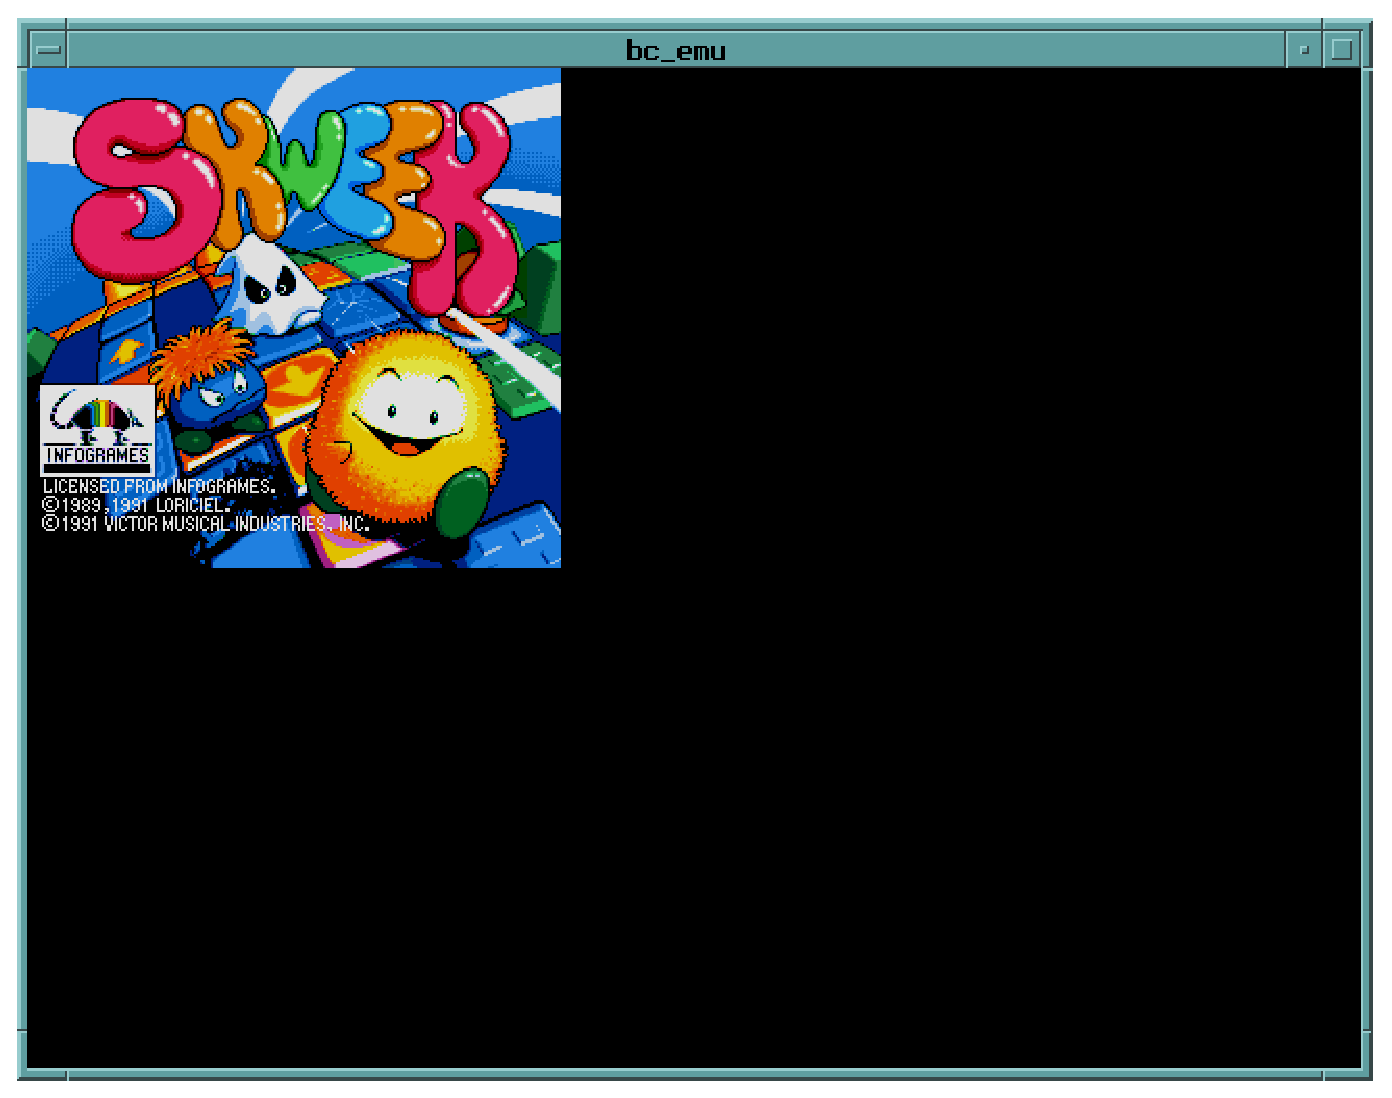
\includegraphics[width=11cm,height=8.5cm]{fig/impl_sdl}
\caption{Obrazovka programu, modul uživatelského rozhraní
	\uv{sdl}\label{fig:impl_sdl}}
\end{center}
\end{figure}

% -----------------------------------------------------------------------------
% Modul uzivatelskeho rozhrani libSDL OpenGL
% -----------------------------------------------------------------------------

\section{Modul uživatelského rozhraní libSDL s podporou
OpenGL}\label{chap:impl_sdlgl}

Modul uživatelského rozhraní libSDL s podporou OpenGL byl naimplementován pro
odlazení a ověření funkčnosti programu s více moduly. Jeho parametry i
používání jsou naprosto identické s původním modulem uživatelského rozhraní
libSDL. Jediným rozdílem je, v případě tohoto modulu, použití akcelerovaného
rozhraní OpenGL pro zobrazování obrazových dat.

Obsah struktury {\em t\_video} je použit jako textura roviny vykreslené přes
celé okno programu (640x480 pixelů) s efektem rozmazání. Snímek obrazovky
s výstupem emulace herního programu {\em Pc Genjin 2} je zobrazen na obr.
~\ref{fig:impl_sdlgl}.

\begin{figure}[ht]
\begin{center}
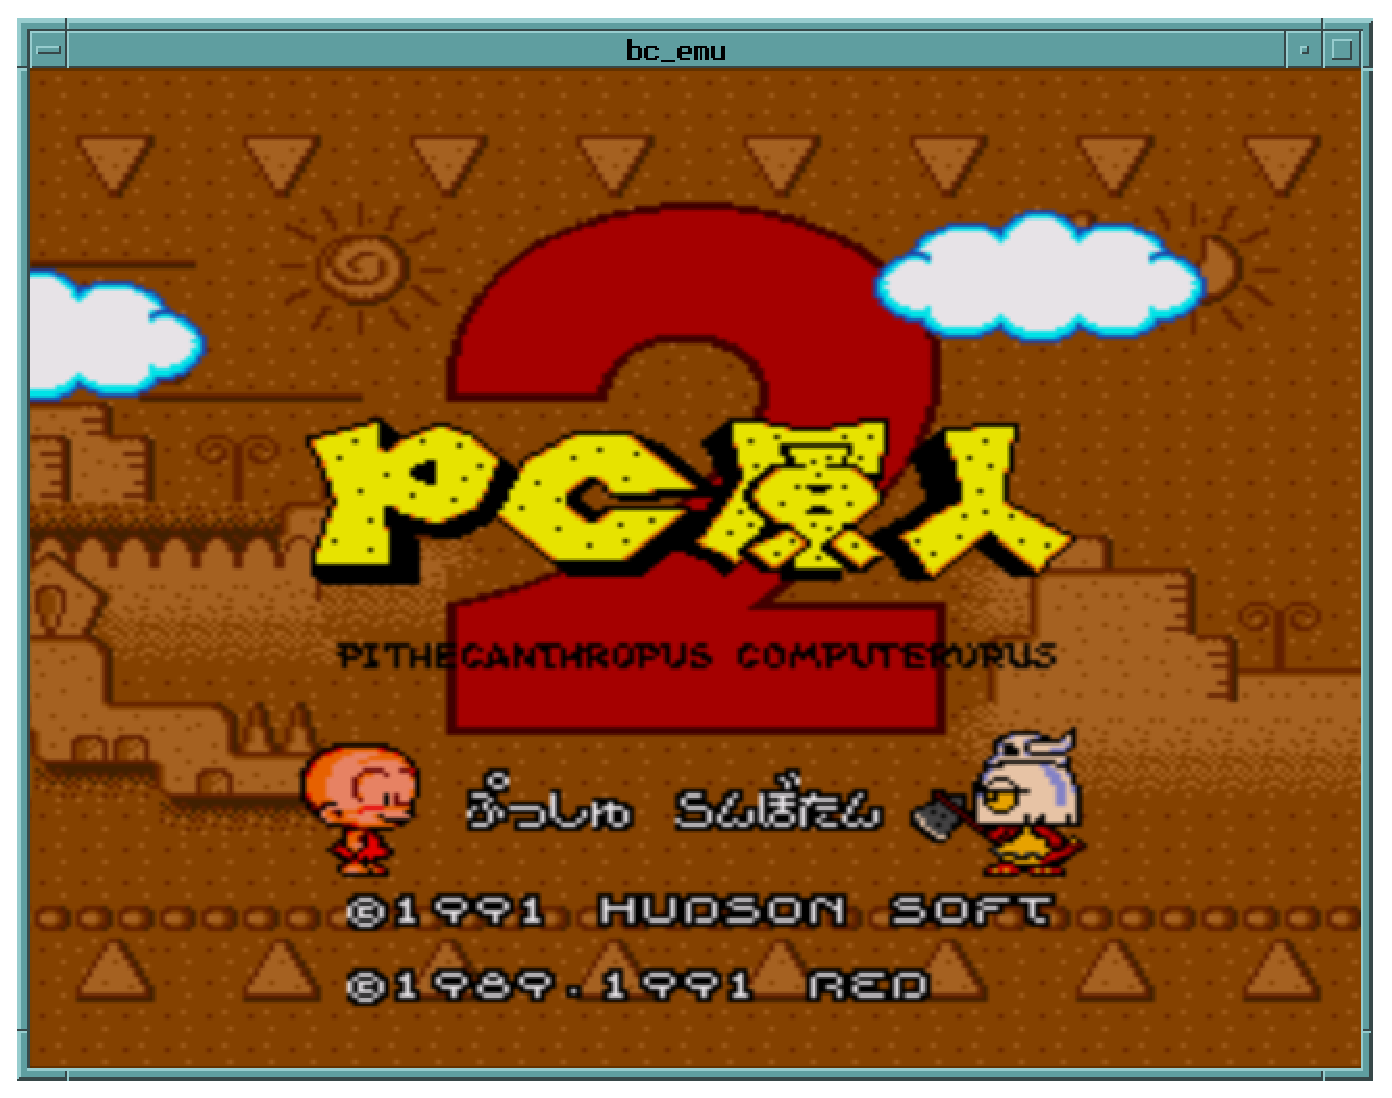
\includegraphics[width=11cm,height=8.5cm]{fig/impl_sdlgl}
\caption{Obrazovka programu, modul uživatelského rozhraní
	\uv{sdlgl}\label{fig:impl_sdlgl}}
\end{center}
\end{figure}

% -----------------------------------------------------------------------------
% Sestavovaci system CMake
% -----------------------------------------------------------------------------

\section{Sestavovací systém CMake}\label{chap:impl_cmake}

Jedním z nefunkčních požadavků na program je {\em přenositelnost kódu}, s čímž
je neodmyslitelně spojen i překlad. Tento úkol velice usnadňuje použitý
sestavovací systém CMake~\cite{wwwCMake} vyvinutý společností Kitware.

CMake slouží jako prostředník při překladu zdrojového kódu (napsaného hlavně v
jazycích C a C++). Na základě platformně nezávislého definičního souboru {\tt
CMakeLists.txt} generuje platformně závislou konfiguraci pro překlad a
sestavení programu. Program tedy může být přeložen běžně dostupnými nástroji
příslušné platformy. CMake podporuje nejběžnější platformy a kromě
definičních souborů {\tt Makefile} dokáže generovat i projektové soubory pro
nejpoužívanější vývojová prostředí Eclipse, KDevelop nebo Microsoft Visual
Studio.

Díky možnosti používání proměnných a testů v rámci zmíněného definičního
souboru {\tt CMakeLists.txt} je možné vytvořit sestavovací prostředí umožňující
jak zavedení platformních restrikcí (sestavení a připojení některého z modulů
jen na určité platformě), tak možnost personifikace sestavení začleněním pouze
určitých modulů zvolených uživatelem.

Sestavení programu je ovlivněno řadou proměnných systému CMake, z nichž většinu
nastavují testy tímto systémem prováděné. V tabulce~\ref{tab:build_opts} je pro
úplnost uveden seznam nejdůležitějších uživatelských proměnných ovlivňujících
sestavení programu včetně jejich významu.

\begin{table}[ht]
\begin{center}
\begin{tabular}{|l|l|c|}
\hline
\textbf{Proměnná} & \textbf{Význam} & \textbf{Hodnota} \\
\hline
{\tt DEBUG} & sestavení vhodné pro lazení & {\tt OFF} \\
{\tt ARCH} & cílová architektura sestavení (v současné době jen \uv{pc}) & {\tt
pc} \\
{\tt EMU\_PCE} & začlenění modulu emulátoru NEC PCEngine & {\tt ON} \\
{\tt UI\_SDL} & začlenění modulu uživ. rozhraní libSDL & {\tt ON} \\
{\tt UI\_SDLGL} & začlenění modulu uživ. rozhraní libSDL s podporou OpenGL & {\tt ON} \\
\hline
\end{tabular}
\end{center}
\caption{Uživatelské proměnné pro konfigurace sestavení pomocí
CMake\label{tab:build_opts}}
\end{table}

